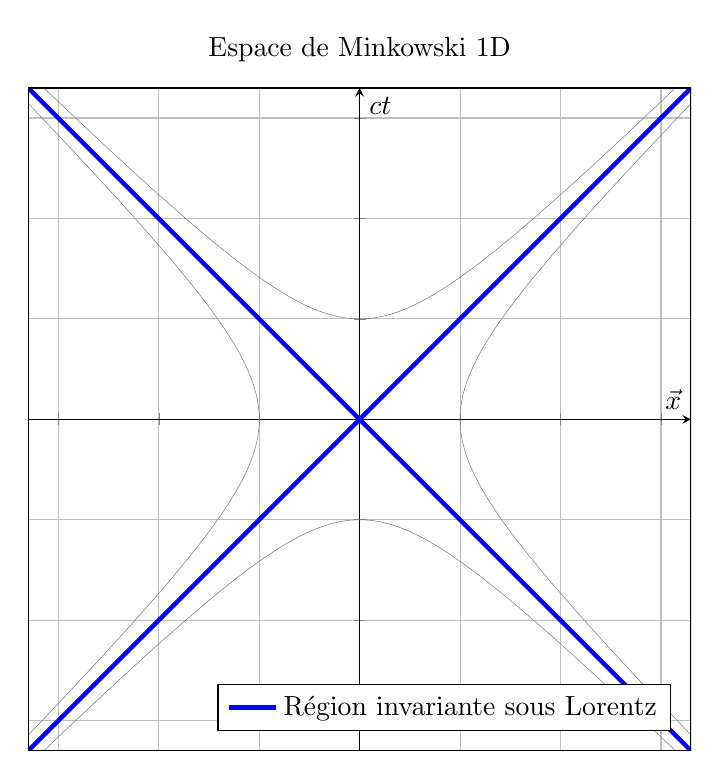
\begin{tikzpicture}
  \begin{axis}[
      samples=121, %nbre de points dans courbes parametrees
      xmin=-3,
      xmax=3,
      ymin=-3,
      ymax=3,
      width=10cm, %taille de la figure
      height=10cm,
      disabledatascaling,
      grid=both, %afficher la grille
      %font=\footnotesize, %taille de la police par defaut
      %grid style={line width=.1pt, draw=red},
      %major grid style={line width=.2pt,draw=gray!50},
      %minor tick num=1,
      axis lines=middle,enlargelimits=0.05, %rendre le plot un rien plus grand
      %execute at begin axis={
      execute at end axis={ %cadre autour
        \draw[thick] (rel axis cs:0,0) -- (rel axis cs:1,0) -- (rel axis cs:1,1) -- (rel axis cs:0,1) --cycle;},
      xticklabels={}, %masquer les nombres en x
      yticklabels={},
      ylabel={$ct$},
      xlabel={$\vec{x}$},
      title={Espace de Minkowski $1$D},
      legend pos=south east,
    ]

    \addplot[ultra thick, blue] expression {x};
    \addplot[ultra thick, blue] expression {-x};
    \legend{Région invariante sous Lorentz}

    \addplot [help lines, domain=-1.9:1.9] ({cosh(x)}, {sinh(x)});
    \addplot [help lines, domain=-1.9:1.9] ({-cosh(x)}, {sinh(x)});
    \addplot [help lines, domain=-1.9:1.9] ({sinh(x)}, {cosh(x)});
    \addplot [help lines, domain=-1.9:1.9] ({sinh(x)}, {-cosh(x)});
  \end{axis}
\end{tikzpicture}
